%% Version 6.1, 1 September 2021
%
%%%%%%%%%%%%%%%%%%%%%%%%%%%%%%%%%%%%%%%%%%%%%%%%%%%%%%%%%%%%%%%%%%%%%%
% amspaperV6.tex --  LaTeX-based instructional template paper for submissions to the 
% American Meteorological Society
%
%%%%%%%%%%%%%%%%%%%%%%%%%%%%%%%%%%%%%%%%%%%%%%%%%%%%%%%%%%%%%%%%%%%%%
% PREAMBLE
%%%%%%%%%%%%%%%%%%%%%%%%%%%%%%%%%%%%%%%%%%%%%%%%%%%%%%%%%%%%%%%%%%%%%

%% Start with one of the following:
% 1.5-SPACED VERSION FOR SUBMISSION TO THE AMS
\documentclass{ametsocV6.1}

% TWO-COLUMN JOURNAL PAGE LAYOUT---FOR AUTHOR USE ONLY
% \documentclass[twocol]{ametsocV6.1}

%%%%%%%%%%%%%%%%%%%%%%%%%%%%%%%%

%%% To be entered by author:

%% May use \\ to break lines in title:

\title{Prithvi-P: Integrating Satellite Observations into an Atmospheric AI Foundation Model for Precipitation Forecasting}

\usepackage{booktabs}

%% Enter authors' names and affiliations as you see in the examples below.
%
%% Use \correspondingauthor{} and \thanks{} (\thanks command to be used for affiliations footnotes, 
%% such as current affiliation, additional affiliation, deceased, co-first authors, etc.)
%% immediately following the appropriate author.
%
%% Note that the \correspondingauthor{} command is NECESSARY.
%% The \thanks{} commands are OPTIONAL.
%
%% Enter affiliations within the \affiliation{} field. Use \aff{#} to indicate the affiliation letter at both the
%% affiliation and at each author's name. Use \\ to insert line breaks to place each affiliation on its own line.

\authors{
  Simon Pfreundschuh\aff{a}\correspondingauthor{Simon Pfreundschuh, simon.pfreundschuh@colostate.edu},
  Christian D. Kummerow\aff{a},
  Jackson Tan\aff{b, c},
  George J. Huffman\aff{c}
}

\affiliation{
  \aff{a}{Colorado State University, Fort Collins, USA}\\
  \aff{b}{University of Maryland, Baltimore County, Baltimore, Maryland, USA} \\
  \aff{c}{NASA Goddard Space Flight Center, Greenbelt, Maryland}
}

%%%%%%%%%%%%%%%%%%%%%%%%%%%%%%%%%%%%%%%%%%%%%%%%%%%%%%%%%%%%%%%%%%%%%
% ABSTRACT
%
% Enter your abstract here
% Abstracts should not exceed 250 words in length!
%

\abstract{%
}

\begin{document}


%% Necessary!
\maketitle

%%%%%%%%%%%%%%%%%%%%%%%%%%%%%%%%%%%%%%%%%%%%%%%%%%%%%%%%%%%%%%%%%%%%%
% SIGNIFICANCE STATEMENT/CAPSULE SUMMARY
%%%%%%%%%%%%%%%%%%%%%%%%%%%%%%%%%%%%%%%%%%%%%%%%%%%%%%%%%%%%%%%%%%%%%
%
% If you are including an optional significance statement for a journal article or a required capsule summary for BAMS 
% (see www.ametsoc.org/ams/index.cfm/publications/authors/journal-and-bams-authors/formatting-and-manuscript-components for details), 
% please apply the necessary command as shown below:
%
% Significance Statement (all journals except BAMS)
%
\statement



%%%%%%%%%%%%%%%%%%%%%%%%%%%%%%%%%%%%%%%%%%%%%%%%%%%%%%%%%%%%%%%%%%%%%
% MAIN BODY OF PAPER
%%%%%%%%%%%%%%%%%%%%%%%%%%%%%%%%%%%%%%%%%%%%%%%%%%%%%%%%%%%%%%%%%%%%%
%
\section{Introduction}
\label{sec:intro}


Precipitation is central to human life and activity: it sustains freshwater
resources, underpins agriculture and energy systems, and drives extreme events
that can threaten lives and economies. Yet it remains one of the most
challenging variables to predict by numerical weather prediction (NWP) models
(Cuo et al., 2011), owing to the complex microphysical processes involved in its
formation (Clark et al., 2016), high spatiotemporal variability (Sukovich et
al., 2014), and poor representation in the initial states of NWP models (Li et
al., 2022).

Given the challenges that conventional weather forecasting systems encounter
with precipitation, there is great potential for AI-based weather prediction
(AIWP) models to address these challenges. AI-based weather forecasting has made
important advances in the last year and a range of models now exceeds
conventional baselines by a significant margin (Lang et al., 2024a).

However, precipitation has received comparably little attention in recently
proposed AIWP models targeting short-to medium-range (1 to 10 day) forecasts. In
fact, not all models include precipitation in their in- and output variables.
While precipitation is included in the output of the AIFS (Lang et al., 2024b),
FourCastNet (Pathak et al., 2022), GenCast (Price et al., 2024a), and FuXi
(Zhong et al., 2024) it is not included in outputs of Stormer (Nguyen et al.,
2024) and Pangu Weather (Bi et al., 2022). For shorter lead time up to twelve
hours, several AI-based now-casting models have been developed that target lead
times up to twelve hours (Agrawal et al., 2025). Due to the difficulty of
accurately representing precipitation in the initial conditions used for NWP
models, nowcasting models typically use radar-based precipitation estimates or
satellite observations as input data for the forecast.

Recent work on AIWP models largely assesses forecast accuracy using test data
that is temporally independent but stems from the same dataset used for training
(Bi et al., 2022; Lang et al.Precipitation is central to human life and
activity: it sustains freshwater resources, underpins agriculture and energy
systems, and drives extreme events that can threaten lives and economies. Yet it
remains one of the most challenging variables to predict by numerical weather
prediction (NWP) models (Cuo et al., 2011), owing to the complex microphysical
processes involved in its formation (Clark et al., 2016), high spatiotemporal
variability (Sukovich et al., 2014), and poor representation in the initial
states of NWP models (Li et al., 2022).

Given the challenges that conventional weather forecasting systems encounter
with precipitation, there is great potential for AI-based weather prediction
(AIWP) models to address these challenges. AI-based weather forecasting has made
important advances in the last year and a range of models now exceeds
conventional baselines by a significant margin (Lang et al., 2024a).

However, precipitation has received comparably little attention in recently
proposed AIWP models targeting short-to medium-range (1 to 10 day) forecasts. In
fact, not all models include precipitation in their in- and output variables.
While precipitation is included in the output of the AIFS (Lang et al., 2024b),
FourCastNet (Pathak et al., 2022), GenCast (Price et al., 2024a), and FuXi
(Zhong et al., 2024) it is not included in outputs of Stormer (Nguyen et al.,
2024) and Pangu Weather (Bi et al., 2022). For shorter lead time up to twelve
hours, several AI-based now-casting models have been developed that target lead
times up to twelve hours (Agrawal et al., 2025). Due to the difficulty of
accurately representing precipitation in the initial conditions used for NWP
models, nowcasting models typically use radar-based precipitation estimates or
satellite observations as input data for the forecast.

Recent work on AIWP models largely assesses forecast accuracy using test data
that is temporally independent but stems from the same dataset used for training
(Bi et al., 2022; Lang et al., 2024b; Nguyen et al., 2024; Pathak et al., 2022;
Price et al., 2024b; Zhong et al., 2024). This implicitly assumes that both the
reference data and the input data used to initialize the forecast accurately
represent the state of the earth system. However, this assumption generally does
not hold for precipitation since it (a) it isn’t well represented in the initial
states of operational weather models and (b) the reanalysis datasets used as
training targets for most AIWP models do not accurately represent precipitation.

In an effort to address some of the shortcomings of existing AIWP models with
respect to precipitation, this work explores the use of the Prithvi-WxC AI
foundation model (FM) for the atmosphere (Schmude et al., 2024) for
precipitation forecasting. We propose Prithvi-Precip, a global precipitation
forecast model based on the Prithvi-WxC AI FM. Prithvi-Precip directly ingests
satellite radiances from a wide range of meteorological sensors in an effort to
to address shortcomings of the analysis in representing precipitation-relevant
processes. Moreover, we show that training forecast models on satellite-derived
global precipitation fields, which — as we will show below — provide a more
accurate precipitation reference especially for convectively driven
precipitation. We evaluate Prithvi-Precip against independent precipitation
estimates from ground-based radars over CONUS demonstrating its potential to
significantly improve upon conventional forecasts using the same operational
forecasting pipeline.


\section{Methods and Data}

\label{sec:methods}

\subsection{The Prithvi-WxC AI Foundation Model}

The Prithvi-WxC AI FM (Schmude et al., 2024) is a transformer-based global
geophysical AI foundation model (). The model has been pre-trained using the
Modern-Era Retrospective Analysis for Research and Applications, version 2
(MERRA-2) reanalysis dataset. The pretext task used for pre-training consists
of predicting past, present, and future reanalysis state from masked input data.

The model architecture -- which is illustrated in Fig. 1 -- is inspired
by the Hiera (Ryali et al., 2023) and MaxViT (Tu et al., 2022) architectures.
The primary input data consists of dynamic model fields comprising 20
single-level and 10 vertical variables at 14 vertical levels. Static data
comprising the spatial coordinates of the data grid, the climatology for the
targeted lead time, as well as the time difference between the two input time
steps and the targeted lead time, are included as additional inputs. The output
of the model are the anomalies of the 160 dynamic atmospheric fields for the
targeted lead time with respect to climatology.


\begin{figure}[h]
 \centerline{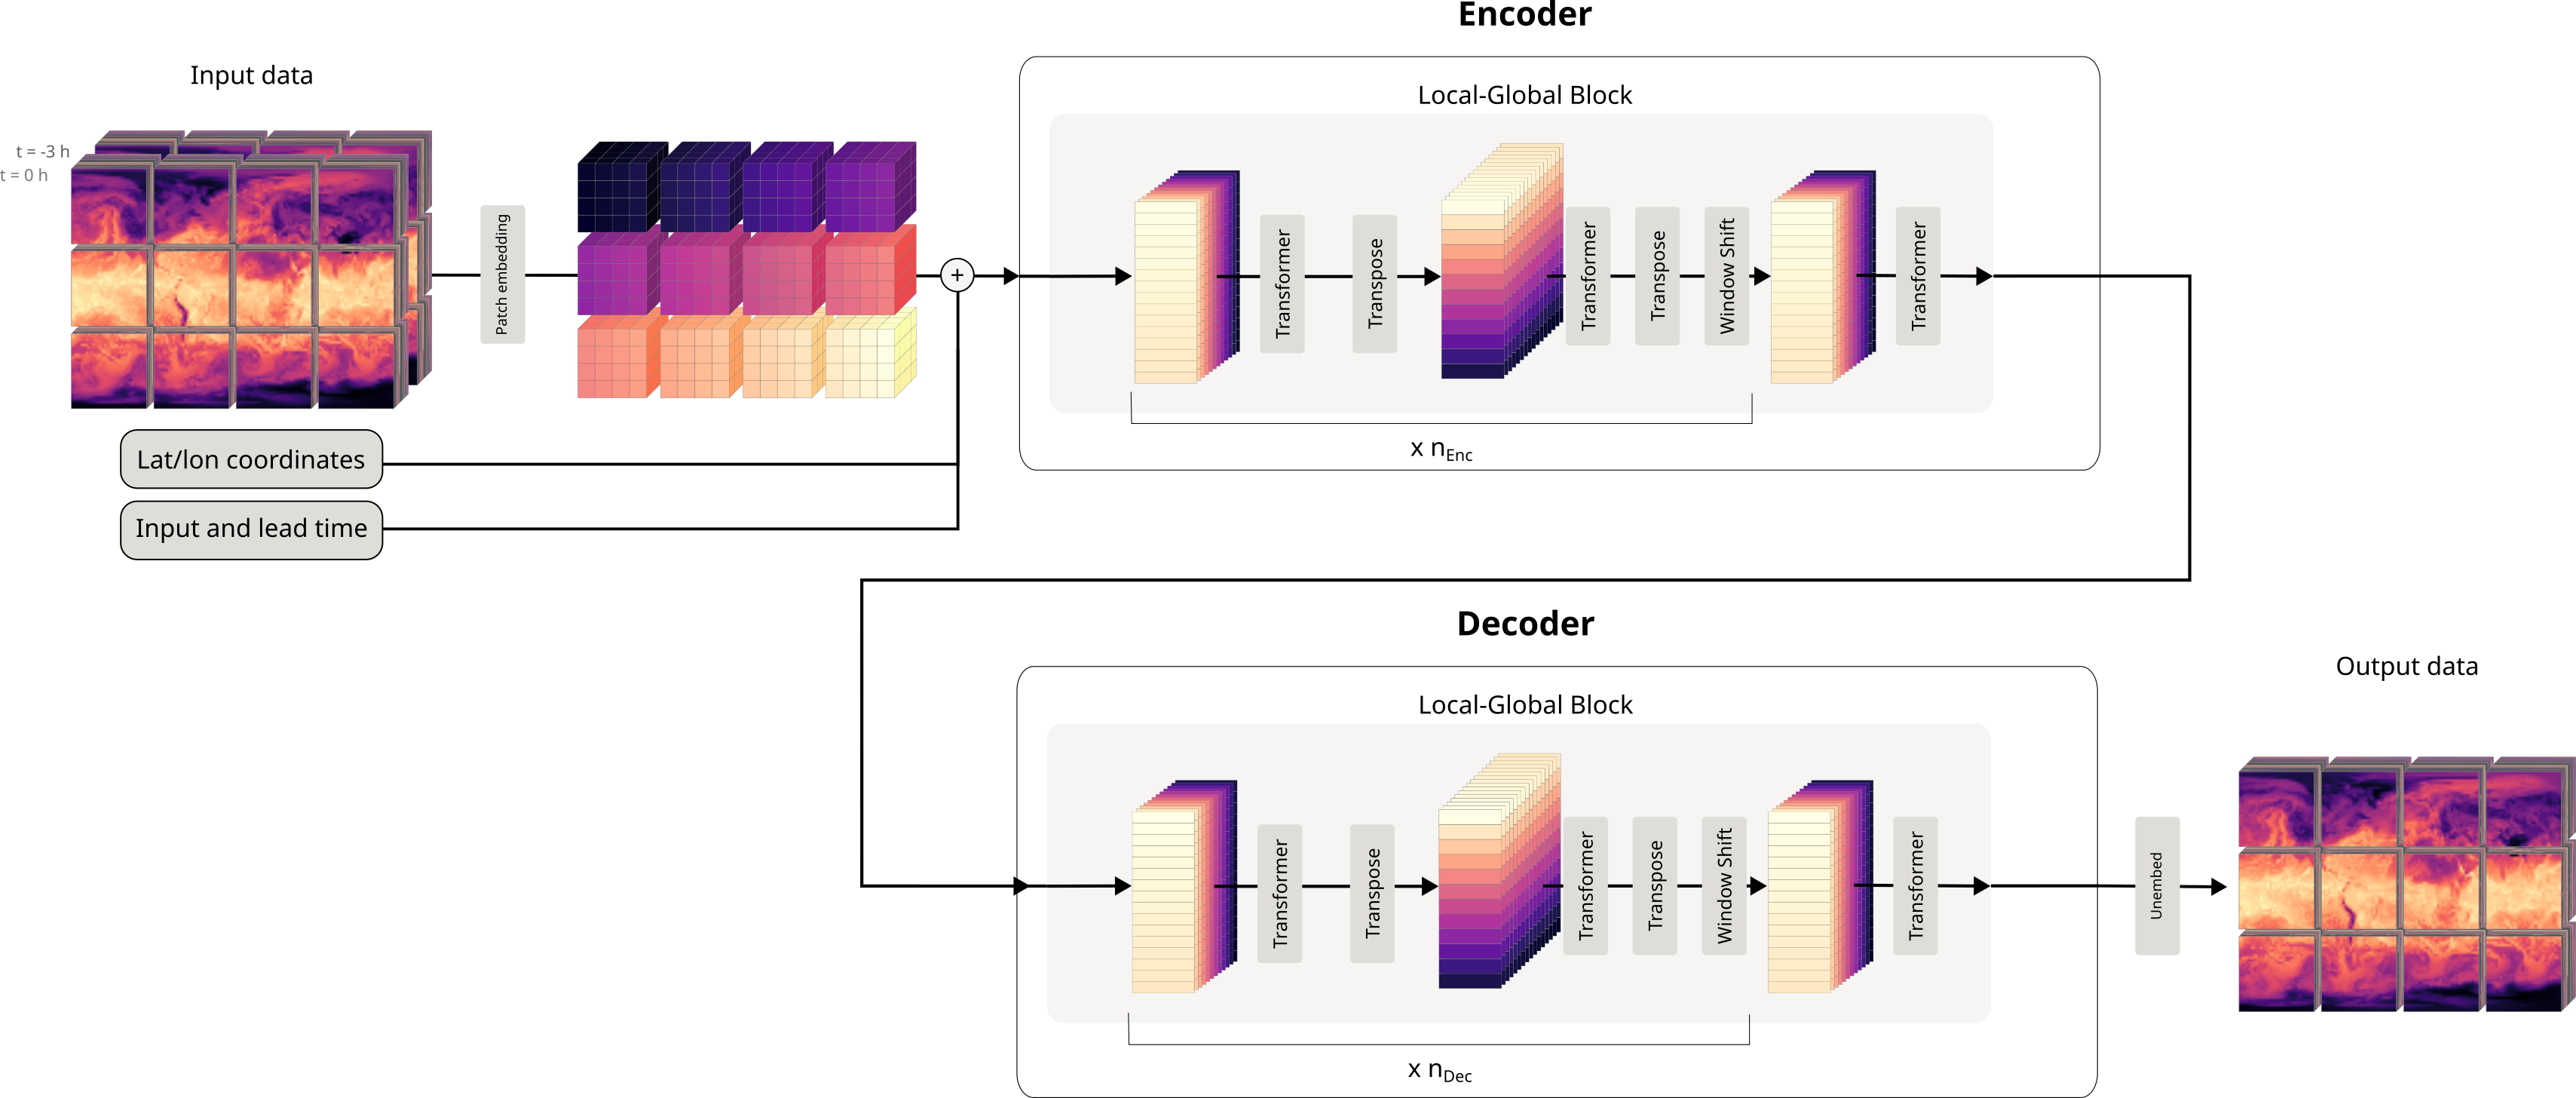
\includegraphics[width=37pc]{figures/figure01.png}}
 \caption{
Architecture of the Prithvi-WxC Foundation Model. The model comprises a transformer-based encoder and decoder. Both components are built from a stack of Local–Global blocks that alternately operate on the latent state within individual spatial tiles and across tiles, enabling information exchange at both local and global scales.
 }\label{fig:prithvi_wxc}
\end{figure}

The pre-training uses the same regular latitude–longitude used by the MERRA-2
reanalysis dataset, which has resolution of 0.67 degree in the zonal dimension
and 0.5 degree in the meridional direction. Internally, the Prithvi-WxC model
splits the input data into horizontal tiles along the zonal and meridional
dimensions. The model alternatingly applies tranformer layers to each tile
independently and the corresponding grid points in each tile to allow for both
local and global information exchange. To avoid tiling artifacts, the model
additionally applies shifting in between consecutive tile-local operations
similar to the Swin architecture (Liu et al., 2021).

\subsection{Forecasting Precipitation with the Prithvi-WxC model}

Since precipitation is not an output variable of the Prithvi-WxC model, we
attach an additional head consisting of a four-layer MLP with GELU activation
functions and layer normalization to the unnormalized output of the Prithvi-WxC
decoder. This modified version of the Prithvi-WxC model thus produces two
outputs, the original MERRA-2 atmospheric state at the requested lead time
together with a 2D global precipitation field. Although the model is finetuned
to predict precipitation, the MERRA-2 atmospheric state is retained to enable
predictions using rollout.

\subsection{Integrating Satellite Observations}


A central challenge for integrating satellite observations into an AIWP model is
the heterogeneity of the observations. The record of meteorological satellite
observations is derived from a diverse set of sensors that have evolved over
decades of satellite remote sensing, each providing measurements with different
channel counts, spectral characteristics, spatial resolutions and sampling. This
diversity poses a fundamental difficulty for conventional machine-learning
approaches, which typically assume a fixed set of input features for model
inputs. In addition, satellite observations are spatially sparse and temporally
irregular at the global scale.

Figure~\ref{fig:observations} illustrates the challenges of integrating
heterogeneous satellite observations into AIWP models using representative
examples from three classes of meteorological satellite sensors. Geostationary
satellites remain at a fixed position relative to the surface of the Earth,
which allows them to continuously observe much of the hemisphere below them. In
contrast, polar-orbiting satellites sample the entire globe through successive,
shifting swaths with limited instantaneous coverage. Finally, specialized
science instruments —such as the GPM Microwave Imager aboard the Global
Precipitation Measurement (GPM) (Draper et al., 2015) — offer still narrower
swaths but deliver higher-resolution and more information-rich measurements than
most operational meteorological sensors.

\begin{figure}[h]
 \centerline{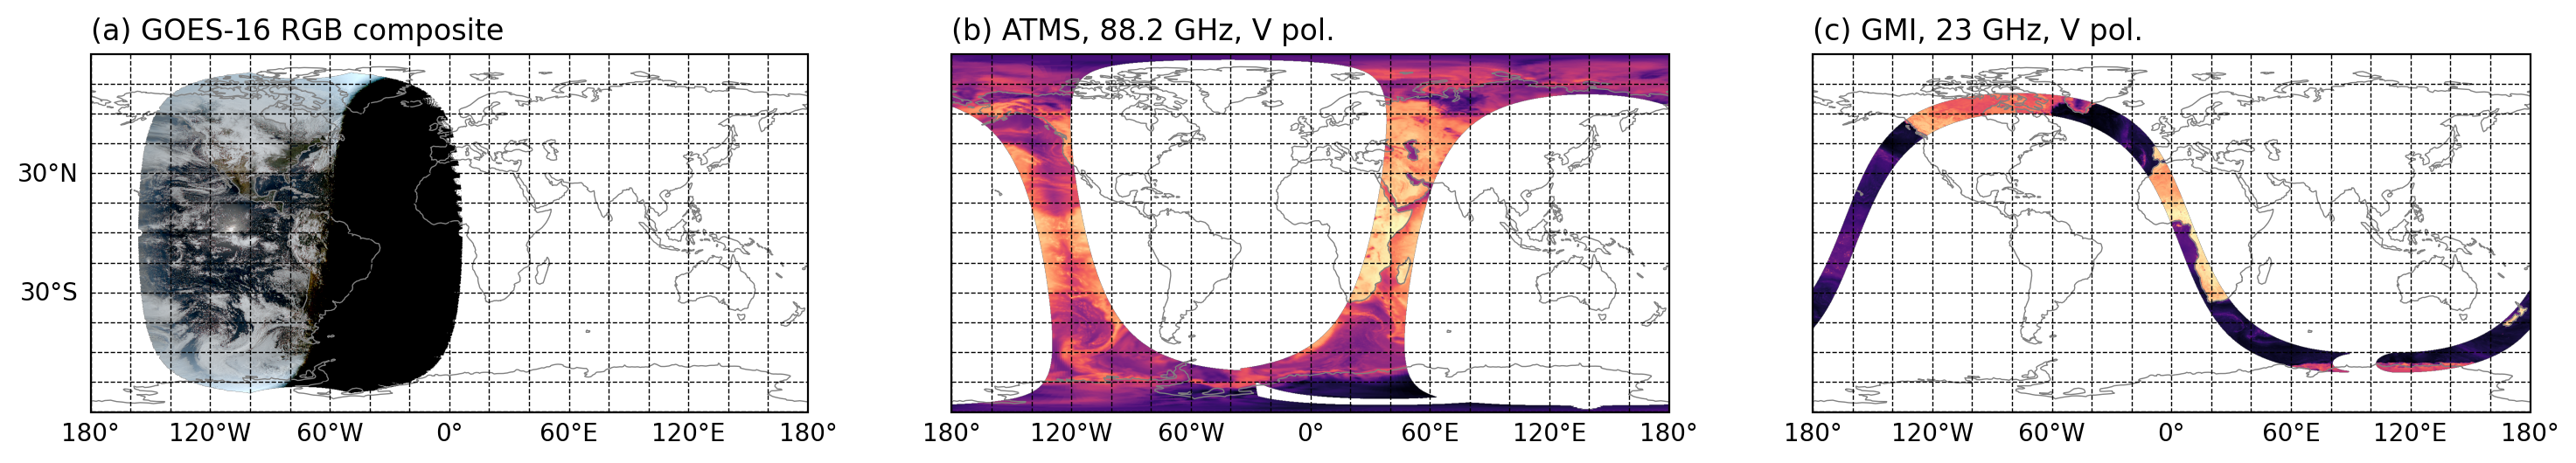
\includegraphics[width=37pc]{figures/figure02.png}}
 \caption{
Examples of meteorological satellite observations from three different sensors.
Panel (a) shows an RGB composite from the Advanced Baseline Imager on the
GOES-16 geostationary satellite. Panel (b) shows quasi-vertically polarized
observations from the 88.2 GHz channels of the Advanced Technology Microwave
Sensor. Panel (c ) shows vertically polarized observations from the 23-GHz
channel on the GPM Microwave Imager (GMI).
 }\label{fig:prithvi_wxc}
\end{figure}


In order to integrate satellite observations into the Prithvi-WxC model in a
generalized fashion, each sensor channel is handled as a separate observation
layer. Furthermore, to handle the sparsity of the observations on the
latitude--longitude grid employed by the Prithvi-WxC model, observations
are stored as tiles matching the internal tiling of the Prithvi-WxC model and
empty tiles are discared. Using this unified approach allows us to build an extensive
observation record across sensor generations and observations. The sensors used
to build the observation input data are listed in Table 1.


\subsubsection{Observation Encoder}

To incorporate the observations into the Prithvi-WxC model, an observation
encoder is added to the model. The observation encoder -- displayed in Fig. 3 --
encodes observations at each tile independently, mapping the variable-length
sequence of observation layers available at each tile to a fixed-sixe latent
space. To allow the observation encoder to distinguish between different
observation layers, the wavelength, polarization, and observation time relative
to a three-hour input window are provided as additional input to each
observation layer. The observations, metadata, and mask in each tile are encoded
into observation tokens with a patch size of 6 x 4 pixels. The large patch size
was chosen to reduce the memory footprint required by the observation encoder
while the asymmetry is due to the tile size used by the Prithvi-WxC model which
prohibits downsampling by a factor of 4 along both height and width. The
arbitrary-length sequences of observation layers are then combined with the
corresponding metadata and encoded into a fixed-dimensional latent space using
cross-attention with single learnable query similar to the approach used in the
Perceiver architecture (cite). The encoded observations from the two input
timesteps are then combined using a temporal encoder and upscaled to match the
token size used internally by the Prithvi-WxC model.

The encoded observations are then merged with the encoded atmospheric state of
the Prithvi-WxC model. This is done using a two-layer MLP that takes the encoded
atmospheric state concatenated with the encoded observations and the current
unrolling step and calculates a residual correction that is added to the encoded
atmospheric state. The resulting architecture of the Prithvi-WxC Precip model is
shown in Fig. 4.

\subsection{Training}

The Prithvi-Precip model is initialized using the weights of Prithvi-WxC model
and trained using the same MERRA-2 input data used for pretraining.
Precipitation estimates from MERRA-2 and the Integrated Multi-Satellite
Retrievals for GPM (IMERG) datasets downsampled to the spatial resolution of the
MERRA-2 grid and a temporal resolution of 3 h are used as training targets. The
Prithvi-Precip model is trained to predict 32 quantiles of the predictive
distribution of precipitation at each grid point using a quantile loss function
(Pfreundschuh et al., 2018)

To determine the best strategy for performing finetuning the Prithvi-WxC model
for precipitation forecasting, we evaluate two different forecasting strategies:
Rollout and continuous forecasting. For rollout, the model is trained to predict
the atmospheric state at a fixed lead time and the resulting output is used as
input to predict the atmospheric state for the next time step. For continuous
forecasting the model is provided the targeted lead time and  trained to directly
predict precipitation for that lead time.

For autoregressive fine-tuning, the model is trained to forecast precipitation 6
hours ahead and is unrolled over six successive time steps. Model parameters are
optimized using the AdamW optimizer based solely on the precipitation prediction
loss. Training uses data from the years 2000–2020 with an epoch consisting of
10\% of all availabe input timesteps from the training period. The model is
trained for 100 epochs during which the learning rate is linearly warmed up over
the first 5 epochs to $5 \cdot 10^{-4}$, after which it follows a
cosine-annealing schedule with restarts at 13, 26, and 52 epochs. Training the
model like this takes about 30 hours on 16 NVIDIA GH200 GPUs.

For continuous forecasting, the model is trained to predict precipitation up to
96 hours ahead. Sicne continuous forecasting is computationally more efficient,
we only subsample the dataset by a factor of 2 per epoch. During initial
experiments we have observed lead-time dependent overfitting with forecasts of
lead (about 48 h) times starting to overfit while forecasts for shorter lead
times are still improving. We therefore apply aggressive data augmentation for
training the continuous forecasts. More specifically, we apply random zonal
rolling, meridional flips and scaling of the input data. For meridional flips we
also adapt the sign of the meridional wind fields accordingly. For the random
flips and rolls, we keep the longitude and latitude fields unchanged since the
Prithvi-WxC is invariant to these transformations when they match the tile size.

To train the final Prithvi-WxC Precip model with satellite observations, the
model is first fine-tuned using only reanalysis inputs following the procedures
described above. The observation encoder is then added and training is repeated,
initializing all weights from the reanalysis-only model. During this stage, the
encoded reanalysis and observation inputs are each randomly dropped with a
probability of 20\%, ensuring that the resulting model can operate with either
input source alone. Additionally, a layer-wise dropout with a 20\% probability
is applied to the observation layers to further increase robustness to missing
satellite observations. For each forecast, 48 observation layers are randomly
chosen from the observations available for each 3-hours window during the input
data window leading to a total of 192 observations layers across two time steps.


%We consider two different forecasting approaches. Most AIWP models forecast
%future atmospheric states using autoregressive unrolling or rollout, where
%forecasts are produced iteratively by feeding the predicted atmospheric state
%back into the model to predict the subsequent state. As an alternative approach,
%we also consider direct forecasting (referred to as continuous forecasting in
%(Nguyen et al., 2024)) where the forecast is performed directly by conditioning
%on the targeted lead time.

\section{Results}
\label{sec:results}


\section{Summary and Conclusions}
\label{sec:summary_and_conclusions}


\clearpage
%%%%%%%%%%%%%%%%%%%%%%%%%%%%%%%%%%%%%%%%%%%%%%%%%%%%%%%%%%%%%%%%%%%%%
% ACKNOWLEDGMENTS
%%%%%%%%%%%%%%%%%%%%%%%%%%%%%%%%%%%%%%%%%%%%%%%%%%%%%%%%%%%%%%%%%%%%%
\acknowledgments

The work of SP and CDK was supported by NASA grant 80NSSC22K0604.

This study uses modified Copernicus Climate Change Service information. Neither the European Commission nor ECMWF is responsible for any use that may be made of the Copernicus information or data it contains.


\datastatement


The NOAA CPC 4-km gridded IR observations are available from \citet{ncep_cpc_mergir_v1}.

The GPM 2BCMB data are available  from \citet{cmb_data}.

The SatRain dataset is available from \citet{satrain_dataset}.

The OceanRAIN data are available from \citet{ocean_rain_data}.

The ERA5 data are available from \citet{c3s_era5_single_levels}.

The GPCP data are available from \citet{gpcp_v33_precip}.



%%%%%%%%%%%%%%%%%%%%%%%%%%%%%%%%%%%%%%%%%%%%%%%%%%%%%%%%%%%%%%%%%%%%%
% APPENDIXES
%%%%%%%%%%%%%%%%%%%%%%%%%%%%%%%%%%%%%%%%%%%%%%%%%%%%%%%%%%%%%%%%%%%%%

%% If only one appendix, use

%\appendix

%% If more than one appendix, use \appendix[<letter>], e.g.,

%\appendix[A] 

%% Appendix title is necessary! For appendix title:

%\appendixtitle{Title of Appendix}

%%% Appendix section numbering (note, skip \section and begin with \subsection)
%
% \subsection{First primary heading}

% \subsubsection{First secondary heading}

% \paragraph{First tertiary heading}



%%%%%%%%%%%%%%%%%%%%%%%%%%%%%%%%%%%%%%%%%%%%%%%%%%%%%%%%%%%%%%%%%%%%%
% REFERENCES
%%%%%%%%%%%%%%%%%%%%%%%%%%%%%%%%%%%%%%%%%%%%%%%%%%%%%%%%%%%%%%%%%%%%%


\bibliographystyle{ametsocV6}
\bibliography{references}


\end{document}
%%%%%%%%%%%%%%%%%%%%%%%%%%%%%%%%%%%%%%%%%%%%%%%%%%%%%%%%%%%%%%%%%%%%%
% END OF AMSPAPERV6.1.TEX
%%%%%%%%%%%%%%%%%%%%%%%%%%%%%%%%%%%%%%%%%%%%%%%%%%%%%%%%%%%%%%%%%%%%%
